\documentclass[aspectratio=169]{beamer}
 
\usetheme{Goettingen}

\usepackage[utf8]{inputenc}
\usepackage[T1]{fontenc}
\usepackage[ngerman]{babel}
\usepackage{graphicx}
\usepackage{listings}
\usepackage{xcolor}
\usepackage{endnotes}
\usepackage[]{hyperref}
\usepackage{pgfplots, relsize}
\pgfplotsset{compat=1.18}
\usepackage{circuitikz}

\lstset{
  language=[LaTeX]TeX, 
  basicstyle=\ttfamily\small,
  keywordstyle=\color{blue},
  commentstyle=\color{gray},
  stringstyle=\color{red},
  showstringspaces=false,
  breaklines=true,
  frame=false,
  numbers=left,
  numberstyle=\tiny\color{gray},
  captionpos=b,
  xleftmargin=2em, 
  framexleftmargin=0.2em,
}



%%%%%%%%%%%%%%%%%%%%%%%%%%%%%%%%%%%%%%%%%%%%%%%%%%%%%%%%%%%%%%%%%%%%%%%%%%%%%%%%
%%%%%%%%%%%%%%%%%%%%%%%%%%%%%%%%%%%%%%%%%%%%%%%%%%%%%%%%%%%%%%%%%%%%%%%%%%%%%%%%
%%%%%%%%%%%%%%%%%%%%%%%%%%%%%%%%%%%%%%%%%%%%%%%%%%%%%%%%%%%%%%%%%%%%%%%%%%%%%%%%


\title{LaTeX Einführung}
\author{Tom Soerr und Ferdinand Grigat}
\date{6.11.2024}

\begin{document}

%%%%%%%%%%%%%%%%%%%%%%%%%%%%%%%%%%%%%%%%%%%%%%%%%%%%%%%%%%%%%%%%%%%%%%%%%%%%%%%%
%%%%%%%%%%%%%%%%%%%%%%%%%%%%%%%%%%%%%%%%%%%%%%%%%%%%%%%%%%%%%%%%%%%%%%%%%%%%%%%%
%%%%%%%%%%%%%%%%%%%%%%%%%%%%%%%%%%%%%%%%%%%%%%%%%%%%%%%%%%%%%%%%%%%%%%%%%%%%%%%%


\begin{frame}
  
\thispagestyle{empty}
\end{frame}




%%%%%%%%%%%%%%%%%%%%%%%%%%%%%%%%%%%%%%%%%%%%%%%%%%%%%%%%%%%%%%%%%%%%%%%%%%%%%%%%
%%%%%%%%%%%%%%%%%%%%%%%%%%%%%%%%%%%%%%%%%%%%%%%%%%%%%%%%%%%%%%%%%%%%%%%%%%%%%%%%
%%%%%%%%%%%%%%%%%%%%%%%%%%%%%%%%%%%%%%%%%%%%%%%%%%%%%%%%%%%%%%%%%%%%%%%%%%%%%%%%


\frame{\titlepage}

\begin{frame}
\frametitle{Gliederung}

\begin{itemize}
  \item Hintergrund
  \item Einführung
  \item Laborbericht
\end{itemize}

% TODO Bild

\end{frame}


%%%%%%%%%%%%%%%%%%%%%%%%%%%%%%%%%%%%%%%%%%%%%%%%%%%%%%%%%%%%%%%%%%%%%%%%%%%%%%%%
%%%%%%%%%%%%%%%%%%%%%%%%%%%%%%%%%%%%%%%%%%%%%%%%%%%%%%%%%%%%%%%%%%%%%%%%%%%%%%%%
%%%%%%%%%%%%%%%%%%%%%%%%%%%%%%%%%%%%%%%%%%%%%%%%%%%%%%%%%%%%%%%%%%%%%%%%%%%%%%%%

\section{Hintergrund}

\subsection{Geschichte}
\begin{frame}
\frametitle{Geschichte}

\begin{itemize}
\item \textbf{1984}: Leslie Lamport entwickelt LaTeX als Makrosystem für TeX.
\item \textbf{Basis}: Auf TeX von Donald Knuth (1978) aufgebaut.
\item \textbf{Ziel}: Wissenschaftliches Schreiben einfacher und strukturierter gestalten.
\end{itemize}

\end{frame}



%%%%%%%%%%%%%%%%%%%%%%%%%%%%%%%%%%%%%%%%%%%%%%%%%%%%%%%%%%%%%%%%%%%%%%%%%%%%%%%%
%%%%%%%%%%%%%%%%%%%%%%%%%%%%%%%%%%%%%%%%%%%%%%%%%%%%%%%%%%%%%%%%%%%%%%%%%%%%%%%%
%%%%%%%%%%%%%%%%%%%%%%%%%%%%%%%%%%%%%%%%%%%%%%%%%%%%%%%%%%%%%%%%%%%%%%%%%%%%%%%%

\subsection{Was ist LaTeX?}
\begin{frame}
\frametitle{Was ist LaTeX?}

\begin{itemize}
\item Programmiersprache für Textsatz
\item LaTeX ist Turing complete
\item WYSIWYM vs. WYSIWYG
\end{itemize}

\end{frame}

%%%%%%%%%%%%%%%%%%%%%%%%%%%%%%%%%%%%%%%%%%%%%%%%%%%%%%%%%%%%%%%%%%%%%%%%%%%%%%%%
%%%%%%%%%%%%%%%%%%%%%%%%%%%%%%%%%%%%%%%%%%%%%%%%%%%%%%%%%%%%%%%%%%%%%%%%%%%%%%%%
%%%%%%%%%%%%%%%%%%%%%%%%%%%%%%%%%%%%%%%%%%%%%%%%%%%%%%%%%%%%%%%%%%%%%%%%%%%%%%%%

\subsection{Wo wird LaTeX eingesetzt?}

\begin{frame}
\frametitle{Wo wird LaTeX eingesetzt?}

\begin{itemize}
\item Wissenschaft
\item Mathematik
\item Informatik
\end{itemize}

\end{frame}

%%%%%%%%%%%%%%%%%%%%%%%%%%%%%%%%%%%%%%%%%%%%%%%%%%%%%%%%%%%%%%%%%%%%%%%%%%%%%%%%
%%%%%%%%%%%%%%%%%%%%%%%%%%%%%%%%%%%%%%%%%%%%%%%%%%%%%%%%%%%%%%%%%%%%%%%%%%%%%%%%
%%%%%%%%%%%%%%%%%%%%%%%%%%%%%%%%%%%%%%%%%%%%%%%%%%%%%%%%%%%%%%%%%%%%%%%%%%%%%%%%

\subsection{Wie funktioniert LaTeX?}

\begin{frame}
\frametitle{Wie funktioniert LaTeX?}

\begin{itemize}
\item LaTeX-Code schreiben
\item LaTeX-Compiler ausführen
\item PDF-Datei erhalten
\end{itemize}

\end{frame}


%%%%%%%%%%%%%%%%%%%%%%%%%%%%%%%%%%%%%%%%%%%%%%%%%%%%%%%%%%%%%%%%%%%%%%%%%%%%%%%%
%%%%%%%%%%%%%%%%%%%%%%%%%%%%%%%%%%%%%%%%%%%%%%%%%%%%%%%%%%%%%%%%%%%%%%%%%%%%%%%%
%%%%%%%%%%%%%%%%%%%%%%%%%%%%%%%%%%%%%%%%%%%%%%%%%%%%%%%%%%%%%%%%%%%%%%%%%%%%%%%%

\section{Einführung}

\subsection{Header}
\begin{frame}[fragile]
\frametitle{Header}

\begin{lstlisting}[language={[latex]TeX}]
\documentclass{beamer}
\usetheme{Goettingen}

\usepackage[utf8]{inputenc}
\usepackage[ngerman]{babel}
\usepackage{listings}
\end{lstlisting}

\vspace{1em}

\begin{itemize}
  \item Pakete importieren
  \item Erscheinungsbild festlegen
\end{itemize}

\end{frame}

%%%%%%%%%%%%%%%%%%%%%%%%%%%%%%%%%%%%%%%%%%%%%%%%%%%%%%%%%%%%%%%%%%%%%%%%%%%%%%%%
%%%%%%%%%%%%%%%%%%%%%%%%%%%%%%%%%%%%%%%%%%%%%%%%%%%%%%%%%%%%%%%%%%%%%%%%%%%%%%%%
%%%%%%%%%%%%%%%%%%%%%%%%%%%%%%%%%%%%%%%%%%%%%%%%%%%%%%%%%%%%%%%%%%%%%%%%%%%%%%%%

\subsection{Sections}
\begin{frame}[fragile]
\frametitle{Sections}

\begin{lstlisting}[language={[latex]TeX}]
\tableofcontents

\section{Hintergrund}
\subsection{Geschichte}
\subsubsection{Entwicklung}
\end{lstlisting}

\vspace{1em}

\begin{itemize}
  \item Automatisch Inhaltsverzeichnis generieren
  \item Gliederung mit Überschriften erstellen
\end{itemize}

\end{frame}

%%%%%%%%%%%%%%%%%%%%%%%%%%%%%%%%%%%%%%%%%%%%%%%%%%%%%%%%%%%%%%%%%%%%%%%%%%%%%%%%
%%%%%%%%%%%%%%%%%%%%%%%%%%%%%%%%%%%%%%%%%%%%%%%%%%%%%%%%%%%%%%%%%%%%%%%%%%%%%%%%
%%%%%%%%%%%%%%%%%%%%%%%%%%%%%%%%%%%%%%%%%%%%%%%%%%%%%%%%%%%%%%%%%%%%%%%%%%%%%%%%

\subsection{Textformatierung}
\begin{frame}[fragile]
\frametitle{Textformatierung}

\begin{lstlisting}[language={[latex]TeX}]
\textbf{Fett} \\
\textit{Kursiv} \\
\underline{Unterstrichen}
\end{lstlisting}

\vspace{1em}

\textbf{Fett} \\
\textit{Kursiv} \\
\underline{Unterstrichen} 

\vspace{1em}

\begin{itemize}
  \item Text hervorheben
\end{itemize}

\end{frame}

%%%%%%%%%%%%%%%%%%%%%%%%%%%%%%%%%%%%%%%%%%%%%%%%%%%%%%%%%%%%%%%%%%%%%%%%%%%%%%%%
%%%%%%%%%%%%%%%%%%%%%%%%%%%%%%%%%%%%%%%%%%%%%%%%%%%%%%%%%%%%%%%%%%%%%%%%%%%%%%%%
%%%%%%%%%%%%%%%%%%%%%%%%%%%%%%%%%%%%%%%%%%%%%%%%%%%%%%%%%%%%%%%%%%%%%%%%%%%%%%%%

\subsection{Aufzählungen}
\begin{frame}[fragile]
\frametitle{Aufzählungen}

\begin{lstlisting}[language={[latex]TeX}]
\begin{itemize}
  \item Erster Punkt
  \item Zweiter Punkt
  \item Dritter Punkt
\end{itemize}
\end{lstlisting}

\vspace{1em}

\begin{itemize}
  \item Erster Punkt
  \item Zweiter Punkt
  \item Dritter Punkt
\end{itemize}

\vspace{1em}

\begin{itemize}
  \item Ungeordnete Liste
\end{itemize}

\end{frame}

%%%%%%%%%%%%%%%%%%%%%%%%%%%%%%%%%%%%%%%%%%%%%%%%%%%%%%%%%%%%%%%%%%%%%%%%%%%%%%%%
%%%%%%%%%%%%%%%%%%%%%%%%%%%%%%%%%%%%%%%%%%%%%%%%%%%%%%%%%%%%%%%%%%%%%%%%%%%%%%%%
%%%%%%%%%%%%%%%%%%%%%%%%%%%%%%%%%%%%%%%%%%%%%%%%%%%%%%%%%%%%%%%%%%%%%%%%%%%%%%%%

\subsection{Mathematische Formeln}

\begin{frame}[fragile]
\frametitle{Mathematische Formeln}

\begin{lstlisting}[language={[latex]TeX}]
$$
\begin{aligned}
  \int_{0}^{\infty} e^{-x^2} \cdot \cos(\pi x) \, dx = \frac{\sqrt{\pi}}{2} e^{-\pi^2/4}
\end{aligned}
$$
\end{lstlisting}

\vspace{1em}

$$
\begin{aligned}
  \int_{0}^{\infty} e^{-x^2} \cdot \cos(\pi x) \, dx = \frac{\sqrt{\pi}}{2} e^{-\pi^2/4}
\end{aligned}
$$

\vspace{1em}


\begin{itemize}
  \item Beste Darstellung mathematischer Formeln
  \item Eingabe ähnlich wie bei viaMINT bzw. Moodle
  \item MathJax für Mathe im Web
\end{itemize}

\end{frame}

%%%%%%%%%%%%%%%%%%%%%%%%%%%%%%%%%%%%%%%%%%%%%%%%%%%%%%%%%%%%%%%%%%%%%%%%%%%%%%%%
%%%%%%%%%%%%%%%%%%%%%%%%%%%%%%%%%%%%%%%%%%%%%%%%%%%%%%%%%%%%%%%%%%%%%%%%%%%%%%%%
%%%%%%%%%%%%%%%%%%%%%%%%%%%%%%%%%%%%%%%%%%%%%%%%%%%%%%%%%%%%%%%%%%%%%%%%%%%%%%%%

\subsection{Bilder}

\begin{frame}[fragile]
\frametitle{Bilder}

\begin{lstlisting}[language={[latex]TeX}]
\begin{figure}
\centering
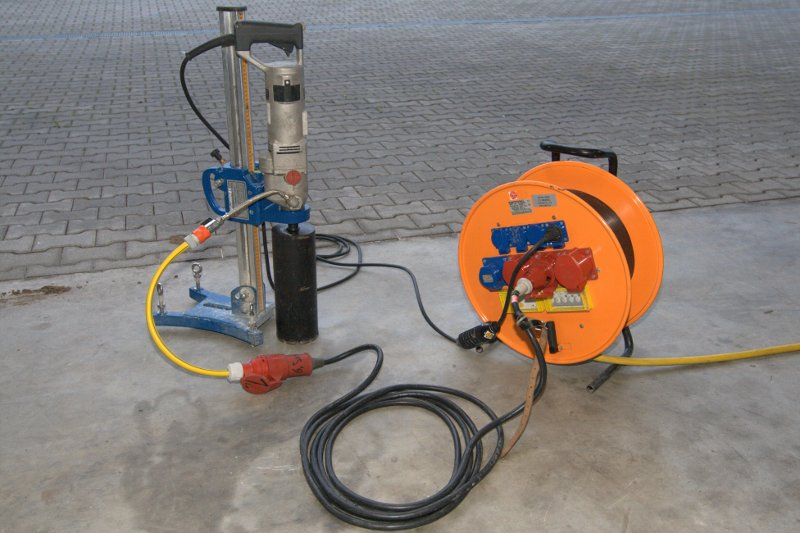
\includegraphics[keepaspectratio]{./assets/image.png}
\end{figure}
\end{lstlisting}

\vspace{1em}

\begin{itemize}
  \item Datei muss mit Pfad angegeben werden
\end{itemize}

\end{frame}

%%%%%%%%%%%%%%%%%%%%%%%%%%%%%%%%%%%%%%%%%%%%%%%%%%%%%%%%%%%%%%%%%%%%%%%%%%%%%%%%
%%%%%%%%%%%%%%%%%%%%%%%%%%%%%%%%%%%%%%%%%%%%%%%%%%%%%%%%%%%%%%%%%%%%%%%%%%%%%%%%
%%%%%%%%%%%%%%%%%%%%%%%%%%%%%%%%%%%%%%%%%%%%%%%%%%%%%%%%%%%%%%%%%%%%%%%%%%%%%%%%

\subsection{Tabellen}

\begin{frame}[fragile]
\frametitle{Tabellen}

\begin{lstlisting}[language={[latex]TeX}]
\begin{table}[H] 
  \centering
  \begin{tabular}{|l|c|r|} 
    \hline
    \textbf{Spalte 1} & \textbf{Spalte 2} & \textbf{Spalte 3} \\ 
    \hline
    Eintrag 1 & Eintrag 2 & Eintrag 3 \\ 
    \hline
  \end{tabular}
\end{table}
\end{lstlisting}

\vspace{1em}

\begin{itemize}
  \item Zeilenumbruch reicht alleine nicht \textbackslash\textbackslash 
  \item Onlinetools nutzen (www.tablesgenerator.com)
\end{itemize}

\end{frame}

\begin{frame}[fragile]
  \frametitle{Tabellen}
  \begin{table}[H] 
    \centering
    \begin{tabular}{|l|c|r|} 
      \hline
      \textbf{Spalte 1} & \textbf{Spalte 2} & \textbf{Spalte 3} \\ 
      \hline
      Eintrag 1 & Eintrag 2 & Eintrag 3 \\ 
      \hline
    \end{tabular}
  \end{table}
\end{frame}

%%%%%%%%%%%%%%%%%%%%%%%%%%%%%%%%%%%%%%%%%%%%%%%%%%%%%%%%%%%%%%%%%%%%%%%%%%%%%%%%
%%%%%%%%%%%%%%%%%%%%%%%%%%%%%%%%%%%%%%%%%%%%%%%%%%%%%%%%%%%%%%%%%%%%%%%%%%%%%%%%
%%%%%%%%%%%%%%%%%%%%%%%%%%%%%%%%%%%%%%%%%%%%%%%%%%%%%%%%%%%%%%%%%%%%%%%%%%%%%%%%

\subsection{Links}

\begin{frame}[fragile]
\frametitle{Links}

\begin{lstlisting}[language={[latex]TeX}]
\href{https://www.google.com}{Google}

Hallo Welt\label{Grafik} \\
Siehe Absatz\ref{Grafik}
\end{lstlisting}

\vspace{1em}

\href{https://www.google.com}{Google}

Hallo Welt\label{Grafik} \\
Siehe Absatz \ref{Grafik}

\vspace{1em}

\begin{itemize}
  \item Weblinks setzen
  \item Referenzen innerhalb des Dokuments setzen und referenzieren
  \item Automatische Nummerierung und Verlinkung
\end{itemize}

\end{frame}

%%%%%%%%%%%%%%%%%%%%%%%%%%%%%%%%%%%%%%%%%%%%%%%%%%%%%%%%%%%%%%%%%%%%%%%%%%%%%%%%
%%%%%%%%%%%%%%%%%%%%%%%%%%%%%%%%%%%%%%%%%%%%%%%%%%%%%%%%%%%%%%%%%%%%%%%%%%%%%%%%
%%%%%%%%%%%%%%%%%%%%%%%%%%%%%%%%%%%%%%%%%%%%%%%%%%%%%%%%%%%%%%%%%%%%%%%%%%%%%%%%

\subsection{Quellenangaben}

\begin{frame}[fragile]

\frametitle{Quellenangaben}


\begin{lstlisting}[language={[latex]TeX}]
\usepackage{endnotes}

Aussage (Google, o. D.) \endnote{\href{https://www.google.com/}{Google. (o. D.). https://www.google.com/}}

\AtEndDocument{\theendnotes}
\end{lstlisting}

\vspace{1em}

Aussage (Google, o. D.) \endnote{\href{https://www.google.com/}{Google. (o. D.). https://www.google.com/}}

\vspace{1em}

\begin{itemize}
  \item Quellenangaben am Ende des Dokuments
  \item Automatische Nummerierung und Verlinkung
\end{itemize}

\end{frame}

%%%%%%%%%%%%%%%%%%%%%%%%%%%%%%%%%%%%%%%%%%%%%%%%%%%%%%%%%%%%%%%%%%%%%%%%%%%%%%%%
%%%%%%%%%%%%%%%%%%%%%%%%%%%%%%%%%%%%%%%%%%%%%%%%%%%%%%%%%%%%%%%%%%%%%%%%%%%%%%%%
%%%%%%%%%%%%%%%%%%%%%%%%%%%%%%%%%%%%%%%%%%%%%%%%%%%%%%%%%%%%%%%%%%%%%%%%%%%%%%%%

\subsection{Grafiken}

\begin{frame}[fragile]
\frametitle{Grafiken}

\begin{figure}[H]\centering

  \begin{tikzpicture}

    \begin{axis}[
      samples=300, % Anzahl der Abtastpunkte
      xmax=8.5, xmin=-8, ymax=4.5, ymin=-4, % Achsengrenzen
      axis lines=left, % Achsenlinien links
      y=0.5cm, x=0.5cm, % Skalierung der Achsen
      grid=both, % Gitterlinien
      xtick={-100,...,100}, ytick={-100,...,100}, % Achsenbeschriftung
      compat=newest,
      xlabel=$x$, xlabel style={at={(1,0)}, anchor=west}, % x-Achsenbeschriftung
      ylabel=$y$, ylabel style={rotate=-90,at={(0,1)}, anchor=south}, % y-Achsenbeschriftung
      every axis plot/.append style={thick} % Linienstil
    ]
      \draw (-50,0) -- (50,0); % x-Achse
      \draw (0,-50) -- (0,50); % y-Achse

      \addplot[blue, domain=-10:10]{4*sin(3*deg(x))}; % Sinuskurve
      \addlegendentry{$f(x)=4\sin(3x)$} % Legende

      \draw[fill] (1,1) circle [radius=2pt]; % Punkt bei (1,1)
      \node[above right] at (1,1) {Punkt}; % Beschriftung des Punktes
      
    \end{axis}
  \end{tikzpicture}

\caption{Sinus Kurve}\label{fig:graph} % Beschriftung und Label
\end{figure}

\end{frame}

%%%%%%%%%%%%%%%%%%%%%%%%%%%%%%%%%%%%%%%%%%%%%%%%%%%%%%%%%%%%%%%%%%%%%%%%%%%%%%%%
%%%%%%%%%%%%%%%%%%%%%%%%%%%%%%%%%%%%%%%%%%%%%%%%%%%%%%%%%%%%%%%%%%%%%%%%%%%%%%%%
%%%%%%%%%%%%%%%%%%%%%%%%%%%%%%%%%%%%%%%%%%%%%%%%%%%%%%%%%%%%%%%%%%%%%%%%%%%%%%%%

\begin{frame}[fragile]
\frametitle{Grafiken}

\begin{figure}[H]\centering % Zentrierte Figur mit fester Position

  \begin{circuitikz}[european] % Europäische Schaltsymbole
    \draw
    (0,0) to[voltage source, v<=$U_q$, a=$10V$] (0,3) % Spannungsquelle
          to[R, l=$R_1$, a=$1\Omega$,i=$I_1$] (3,3) % Widerstand R1
          to[R, l=$R_3$, a=$21\Omega$, i=$I_3$] (6,3) % Widerstand R3
          to[R, l=$R_4$, a=$20\Omega$] (6,0) % Widerstand R4
          -- (3,0)
          -- (0,0);
    \draw
    (3,3) to[short, *-, i>_=$I_2$] (3,2) % Verbindung mit Strom I2
          to[R, l=$R_2$, a=$9\Omega$] (3,1) % Widerstand R2
          to[short, -*] (3,0)
    ;
    \node at (1.5,1.5) {$1$}; % Knoten 1
    \node at (4.5,1.5) {$2$}; % Knoten 2
  \end{circuitikz}

\caption{Schaltkreis}\label{fig:cir} % Beschriftung und Label
\end{figure}

\end{frame}

%%%%%%%%%%%%%%%%%%%%%%%%%%%%%%%%%%%%%%%%%%%%%%%%%%%%%%%%%%%%%%%%%%%%%%%%%%%%%%%%
%%%%%%%%%%%%%%%%%%%%%%%%%%%%%%%%%%%%%%%%%%%%%%%%%%%%%%%%%%%%%%%%%%%%%%%%%%%%%%%%
%%%%%%%%%%%%%%%%%%%%%%%%%%%%%%%%%%%%%%%%%%%%%%%%%%%%%%%%%%%%%%%%%%%%%%%%%%%%%%%%

\section{Laborbericht}

\begin{frame}
\frametitle{Laborbericht}
% insert qr code from ./assets/qr.png
\begin{figure}[H]
  \centering
  \includegraphics[width=0.5\textwidth,keepaspectratio]{./assets/qr.png}
\end{figure}
\end{frame}

%%%%%%%%%%%%%%%%%%%%%%%%%%%%%%%%%%%%%%%%%%%%%%%%%%%%%%%%%%%%%%%%%%%%%%%%%%%%%%%%
%%%%%%%%%%%%%%%%%%%%%%%%%%%%%%%%%%%%%%%%%%%%%%%%%%%%%%%%%%%%%%%%%%%%%%%%%%%%%%%%
%%%%%%%%%%%%%%%%%%%%%%%%%%%%%%%%%%%%%%%%%%%%%%%%%%%%%%%%%%%%%%%%%%%%%%%%%%%%%%%%

\section{Quellen}
\begin{frame}
  \frametitle{Quellen}
  \begin{itemize}
    \item Alle Videos / Edmund Weitz. (o. D.). https://weitz.de/haw-videos/ 
    \item Dokumentation | KOMA-Script Documentation Project. (o. D.). https://komascript.de/book 
    \item Kopka, H. (1991). Latex: eine Einführung. 
    \item PGF/TIKZ Manual - Complete online documentation. (o. D.). https://tikz.dev/ 
    \item Wikipedia contributors. (2024, 29. Oktober). LaTeX. Wikipedia. https://en.wikipedia.org/wiki/LaTeX
  \end{itemize}

\end{frame}

% TODO: PDF abschicken


\end{document}


